\chapter{Représentations de couleur, hadrons et confinement}

\paragraph{Brève digression liminaire.}
Avant de revenir à la théorie des groupes, permettez-moi une publicité éhontée. \emph{La Guerre des trous noirs} raconte la longue controverse avec Stephen Hawking sur la question de savoir si les trous noirs détruisent l’information quantique. Le livre évoque aussi une cruauté propre aux physiciens théoriciens : il n’y a pas que le chat de Schrödinger, il y a aussi le poisson de Susskind et son malheureux voyage dans les toilettes. Cette obligation remplie, revenons à Alice et Bob. Alice souffre toujours, car Bob continue de lui faire apprendre la théorie des groupes.

\lectureoverview{Une symétrie devient physique par son action sur les états. Nous commencerons par les rotations pour introduire les représentations et les générateurs, puis nous reprendrons cette construction pour la couleur \(SU(3)\). Les représentations de couleur se combinent pour former des hadrons, et leur dynamique explique pourquoi on n’observe jamais de couleur isolée.}

\section{Le groupe et les objets sur lesquels il agit}

Toute discussion sur les symétries repose sur deux idées. D’abord, un groupe abstrait : un ensemble d’opérations muni d’une loi de composition, d’un élément neutre et d’inverses. Ensuite, les objets sur lesquels ces opérations agissent. On peut distinguer ces deux idées, mais en physique, elles ne peuvent pas être séparées. Une symétrie importe parce qu’elle transforme des états physiques, des champs, des coordonnées ou des observables.

\begin{classroomqa}
\audiencequestion{On a décrit un groupe à la fois comme une table de multiplication abstraite et comme des matrices agissant sur des objets physiques. Peut-on dissocier ces deux aspects ?
\lecturetimestamp{00:01:58}}
\lecturerresponse{Il s’agit de deux niveaux de description distincts, mais étroitement liés. Une rotation existe comme opération abstraite avant que l’on précise ce qu’elle fait tourner. La physique demande ensuite comment cette même opération agit sur les états et les grandeurs pertinents pour un système donné. Les matrices décrivent cette action concrète tout en préservant la loi de composition abstraite.}
\end{classroomqa}

Les rotations spatiales en offrent l’exemple le plus simple. En mécanique classique, une même rotation peut agir sur les coordonnées d’une particule, sur la direction d’un aimant ou sur tout autre vecteur. En mécanique quantique, les états appartiennent à un espace vectoriel linéaire ; une rotation y est donc représentée par un opérateur linéaire. Si \(g\) désigne un élément abstrait du groupe et \(D(g)\) sa matrice représentative, la cohérence exige que
\begin{equation}
D(g_1g_2)=D(g_1)D(g_2),
\qquad
D(e)=\boldsymbol 1.
\end{equation}
Les matrices n’ont pas besoin de ressembler aux opérations abstraites, mais leur multiplication doit reproduire la loi de composition du groupe.
\editorialnote{L’équation d’homomorphisme explicite la correspondance entre la composition des éléments du groupe et la multiplication des matrices, décrite verbalement dans la source.}

La dimension de la matrice est déterminée par l’espace des états, et non par le seul groupe abstrait. Si l’on ne conserve que le spin d’un électron, il existe deux possibilités orthogonales, le spin vers le haut et le spin vers le bas, et un état est un vecteur colonne à deux composantes. Les rotations agissent donc par des matrices \(2\times2\). Pour deux objets de spin un demi, il existe quatre états de base,
\begin{equation}
\ket{\uparrow\uparrow},\qquad
\ket{\uparrow\downarrow},\qquad
\ket{\downarrow\uparrow},\qquad
\ket{\downarrow\downarrow},
\end{equation}
et l’action induite sur l’espace composé est de dimension quatre.

La suite familière est
\begin{equation}
\begin{array}{c|c|c}
\text{spin} & \text{number of states} & \text{matrix dimension}\\
\hline
0 & 1 & 1\times1\\
\frac12 & 2 & 2\times2\\
1 & 3 & 3\times3\\
\frac32 & 4 & 4\times4
\end{array}
\end{equation}
et ainsi de suite. Un état de spin nul fournit la représentation triviale : toute rotation le laisse inchangé. La matrice un par un est simplement \(1\). Un état de spin un a trois composantes, et ses matrices de rotation sont les rotations vectorielles tridimensionnelles usuelles. Plus généralement, le spin \(j\) comporte \(2j+1\) états.

La représentation peut aussi être de dimension infinie. Si l’on décrit le mouvement orbital complet d’un électron plutôt que son seul spin, un état comprend une amplitude pour chaque position, ou, de façon équivalente, pour chaque impulsion. L’opérateur de rotation agit alors sur un espace de fonctions d’onde de dimension infinie. Ainsi, un même groupe abstrait des rotations possède des représentations triviale, bidimensionnelle, tridimensionnelle et de dimension infinie. C’est ce fait que nous réutiliserons lorsque nous passerons du spin à la couleur.

\section{Pourquoi les rotations de spin sont des matrices unitaires spéciales}

Revenons maintenant au spin d’un électron isolé et écartons son mouvement orbital. Une rotation est représentée par une matrice unitaire \(2\times2\) \(U\),
\begin{equation}
U^\dagger U=\boldsymbol 1,
\qquad
U^{-1}=U^\dagger.
\label{eq:l4-unitarity}
\end{equation}
La transformation inverse doit annuler la rotation et l’unitarité préserve la norme, donc toutes les probabilités.

Une matrice complexe générale \(2\times2\) contient quatre entrées complexes, soit huit paramètres réels. L’équation~\eqref{eq:l4-unitarity} impose quatre conditions réelles indépendantes, ce qui laisse quatre paramètres. Une rotation spatiale ordinaire n’en a que trois : deux paramètres déterminent l’axe et un autre, l’angle. La matrice unitaire comporte donc une phase de trop. La restriction supplémentaire est
\begin{equation}
\det U=1.
\label{eq:l4-det-one}
\end{equation}
Le décompte devient alors
\begin{equation}
8-4-1=3.
\end{equation}

La condition que le déterminant vaille un est préservée par multiplication, car
\begin{equation}
\det(AB)=\det A\,\det B.
\end{equation}
Si deux matrices ont chacune un déterminant égal à un, leur produit aussi. Cette condition est également compatible avec l’unitarité. En prenant le déterminant de l’équation~\eqref{eq:l4-unitarity}, on obtient
\begin{equation}
1=\det(U^\dagger U)
=\det(U^\dagger)\det U
=(\det U)^*\det U.
\end{equation}
Par conséquent, le déterminant d’une matrice unitaire appartient au cercle unité :
\begin{equation}
\det U=e^{i\phi}.
\end{equation}

\begin{classroomqa}
\audiencequestion{L’unitarité exige-t-elle que le déterminant soit réel ?
\lecturetimestamp{00:12:10}}
\lecturerresponse{Non. L’unitarité exige seulement que son module vaille un. Le déterminant peut être une phase quelconque \(e^{i\phi}\). Pour une matrice de dimension deux, multiplier \(U\) par \(e^{-i\phi/2}\) élimine cette phase commune et donne une matrice de déterminant un.}
\end{classroomqa}

En effet, si
\begin{equation}
V=e^{-i\phi/2}U,
\end{equation}
alors \(V\) reste unitaire et
\begin{equation}
\det V=e^{-i\phi}\det U=1.
\end{equation}
Les matrices unitaires de déterminant un forment \(SU(2)\).

Il y a une subtilité. On pourrait être tenté de dire que \(SU(2)\) est simplement le groupe des rotations de l’espace tridimensionnel, mais la correspondance est double. Les matrices \(U\) et \(-U\) agissent différemment sur un spineur, tout en correspondant à la même rotation d’un vecteur ordinaire. Ainsi,
\begin{equation}
SU(2)/\{\boldsymbol 1,-\boldsymbol 1\}\simeq SO(3).
\end{equation}
Pour la discussion présente, ce sont la structure locale de la loi de composition et les trois générateurs qui comptent ; le revêtement double explique toutefois le caractère à deux valeurs des rotations de spin un demi.

\section{Transformations infinitésimales et leurs générateurs}

Une rotation finie peut être construite à partir d’un grand nombre de rotations très petites. Un élément du groupe proche de l’identité est dit infinitésimal et, dans un groupe connexe, connaître toutes les directions infinitésimales suffit à reconstruire les transformations finies par compositions répétées. Plus important encore en physique, les opérateurs qui engendrent ces transformations infinitésimales sont les grandeurs conservées associées à la symétrie.

Écrivons un élément proche de l’identité sous la forme
\begin{equation}
U=\boldsymbol 1+i\epsilon T,
\qquad |\epsilon|\ll1.
\label{eq:l4-infinitesimal-u}
\end{equation}
Le facteur \(i\) relève d’une convention commode. En substituant cette expression dans la condition d’unitarité et en négligeant les termes d’ordre \(\epsilon^2\), on obtient
\begin{align}
(\boldsymbol 1+i\epsilon T)
(\boldsymbol 1-i\epsilon T^\dagger)&=\boldsymbol 1,
\\
i\epsilon(T-T^\dagger)&=0,
\\
T&=T^\dagger.
\label{eq:l4-hermitian-generator}
\end{align}
Le générateur est hermitien, comme doit l’être une observable en mécanique quantique.

\begin{figure}[htbp]
\centering
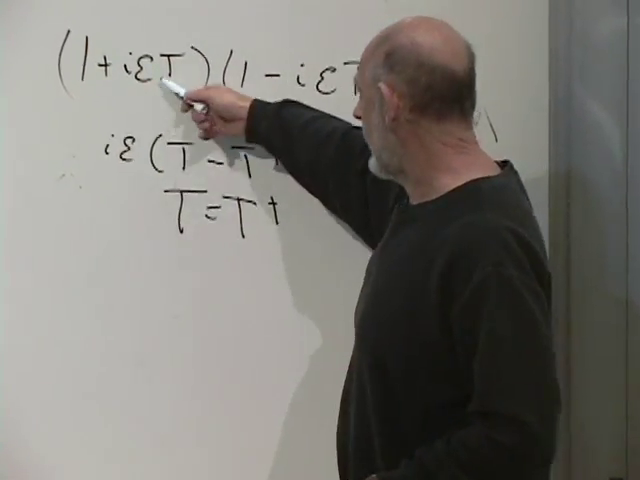
\includegraphics[width=0.62\textwidth]{lecture_04_figure_03.png}
\caption{Le calcul d’unitarité au voisinage de l’identité, qui aboutit à \(T=T^\dagger\).}
\lectureframe{00:23:28}
\end{figure}

Pour les rotations spatiales, il existe trois générateurs linéairement indépendants, car il y a trois axes infinitésimaux indépendants. Une petite rotation autour d’une direction quelconque se compose de petites rotations autour de \(x\), \(y\) et \(z\). Les générateurs correspondants sont les opérateurs de moment cinétique \(J_x,J_y,J_z\). Leurs commutateurs codent la non-commutativité des rotations :
\begin{equation}
[J_i,J_j]=i\epsilon_{ijk}J_k.
\label{eq:l4-angular-momentum-algebra}
\end{equation}
Des rotations infinitésimales répétées construisent alors une rotation finie.

Nous avons utilisé l’unitarité, mais pas encore la condition que le déterminant vaille un. Pour toute petite matrice \(m\),
\begin{equation}
\det(\boldsymbol 1+\epsilon m)
=1+\epsilon\,\operatorname{tr}m+O(\epsilon^2).
\label{eq:l4-det-expansion}
\end{equation}

\begin{figure}[htbp]
\centering
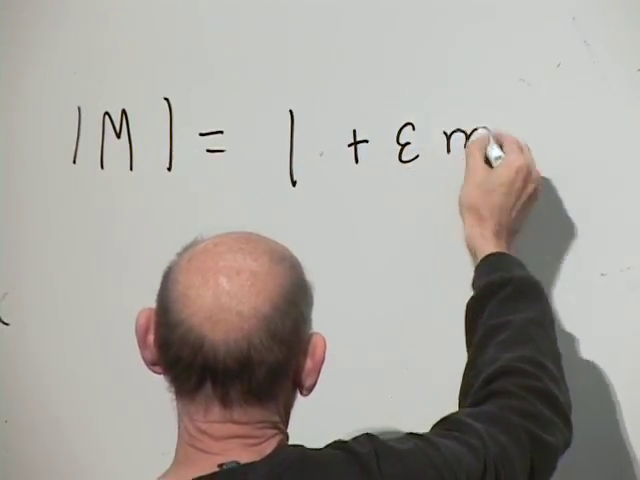
\includegraphics[width=0.62\textwidth]{lecture_04_figure_02.png}
\caption{Le développement du déterminant au premier ordre, tel qu’il commence au tableau.}
\lectureframe{00:21:51}
\end{figure}

En appliquant l’équation~\eqref{eq:l4-det-expansion} à l’équation~\eqref{eq:l4-infinitesimal-u},
\begin{equation}
\det U
=1+i\epsilon\,\operatorname{tr}T+O(\epsilon^2).
\end{equation}
La condition d’unitarité spéciale impose donc
\begin{equation}
\operatorname{tr}T=0.
\label{eq:l4-traceless-generator}
\end{equation}
Les générateurs de \(SU(2)\) sont précisément les matrices hermitiennes sans trace \(2\times2\). Cet espace vectoriel est de dimension trois. Les matrices de Pauli en fournissent une base usuelle :
\begin{equation}
\begin{aligned}
\sigma_x&=
\begin{pmatrix}0&1\\1&0\end{pmatrix},
&
\sigma_y&=
\begin{pmatrix}0&-i\\i&0\end{pmatrix},
\\[0.4em]
\sigma_z&=
\begin{pmatrix}1&0\\0&-1\end{pmatrix}.
\end{aligned}
\end{equation}
Pour une représentation de spin un demi, on peut prendre \(J_i=\sigma_i/2\) ; une rotation finie d’angle \(\theta\) autour de \(\hat{\boldsymbol n}\) est alors donnée par
\begin{equation}
U(\hat{\boldsymbol n},\theta)
=\exp\!\left(-i\theta\,
\hat{\boldsymbol n}\cdot\boldsymbol\sigma/2\right).
\end{equation}
\editorialnote{L’exponentielle finie est le prolongement usuel de la discussion des générateurs infinitésimaux. La source insiste sur les rotations infinitésimales répétées sans écrire explicitement cette formule.}

\begin{classroomqa}
\audiencequestion{Il y a donc trois matrices hermitiennes sans trace indépendantes \(2\times2\) ?
\lecturetimestamp{00:24:07}}
\lecturerresponse{Oui. Ce sont les trois matrices de Pauli. Pour les matrices spéciales unitaires \(3\times3\), leur nombre est huit et une base usuelle est donnée par les huit matrices de Gell-Mann.}
\end{classroomqa}

\begin{classroomqa}
\audiencequestion{Est-ce le même ``huit'' que celui de la voie octuple et des huit gluons ?
\lecturetimestamp{00:24:43}}
\lecturerresponse{Les mathématiques relèvent du même type de théorie des représentations \(SU(3)\), mais il faut préciser quelle symétrie \(SU(3)\) agit. La symétrie de saveur historique de la voie octuple n’est pas la couleur \(SU(3)\). Les huit gluons appartiennent à la représentation adjointe de la couleur \(SU(3)\).}
\end{classroomqa}

\section{De SU(2) à SU(3) de couleur}

Passons maintenant des matrices \(2\times2\) aux matrices \(3\times3\). Une matrice complexe générale \(3\times3\) possède neuf entrées complexes, soit dix-huit paramètres réels. La condition \(U^\dagger U=\boldsymbol 1\) fournit neuf contraintes réelles, et la condition \(\det U=1\) en supprime une de plus. Par conséquent,
\begin{equation}
18-9-1=8.
\end{equation}
Il existe huit directions infinitésimales indépendantes et huit générateurs hermitiens sans trace. Contrairement à \(SU(2)\), ce groupe n’est pas le groupe des rotations de l’espace ordinaire tridimensionnel. C’est une symétrie interne qui agit sur la couleur.

Avant d’attribuer ces représentations aux quarks, rappelons comment apparaissent les représentations composées. Prenons deux systèmes de spin un demi et négligeons leur mouvement orbital. Il existe quatre états produits, mais une rotation ne mélange pas les quatre de manière irréductible. Trois combinaisons se transforment comme un spin un,
\begin{align}
\ket{1,1}&=\ket{\uparrow\uparrow},\\
\ket{1,0}&=\frac{1}{\sqrt2}
(\ket{\uparrow\downarrow}+\ket{\downarrow\uparrow}),\\
\ket{1,-1}&=\ket{\downarrow\downarrow},
\end{align}
tandis que la quatrième se transforme comme un spin nul,
\begin{equation}
\ket{0,0}=\frac{1}{\sqrt2}
(\ket{\uparrow\downarrow}-\ket{\downarrow\uparrow}).
\end{equation}
Ainsi,
\begin{equation}
\boldsymbol 2\otimes\boldsymbol 2
=\boldsymbol 3\oplus\boldsymbol 1.
\label{eq:l4-two-spin-decomposition}
\end{equation}
Les états alignés donnent les états \(m=\pm1\) du triplet ; l’état symétrique de projection nulle le complète, tandis que la combinaison antisymétrique est le singulet. C’est la logique générale de l’addition des moments cinétiques et de la combinaison des représentations de couleur.

La distinction singulet--triplet se retrouve chaque fois que l’on couple deux degrés de liberté de spin un demi. Dans l’hydrogène atomique, les spins de l’électron et du proton forment des états hyperfins singulet et triplet. L’orthohydrogène et le parahydrogène relèvent de la même théorie des représentations pour les spins nucléaires des deux protons d’une molécule \(H_2\).
\editorialnote{La source emploie les termes ``ortho et para-hydrogène'' en évoquant les spins du proton--et de l’électron dans un atome d’hydrogène. La décomposition mathématique est correcte ; les appellations moléculaires et atomiques sont distinguées ici par souci de précision.}

\subsection{Le triplet et l’antitriplet}

Un quark isolé possède trois amplitudes de couleur. Dans une base donnée, écrivons
\begin{equation}
q=
\begin{pmatrix}
q_r\\q_g\\q_b
\end{pmatrix},
\qquad
q'=Uq,
\qquad U\in SU(3).
\label{eq:l4-quark-triplet}
\end{equation}
Les trois entrées peuvent être les amplitudes d’état d’un quark, ou trois opérateurs de champ qui créent des quarks rouges, verts et bleus. Le groupe mélange ces trois composantes. Un état initialement rouge devient généralement une superposition de rouge, de vert et de bleu après une transformation de couleur. Cette représentation fondamentale de dimension trois est appelée \(\boldsymbol 3\).

Pour un antiquark, le groupe agit selon la représentation complexe conjuguée de celle du quark. En prenant le conjugué complexe de l’équation~\eqref{eq:l4-quark-triplet}, on obtient
\begin{equation}
\bar q'=U^*\bar q.
\end{equation}
Cette représentation est notée \(\bar{\boldsymbol 3}\). L’analogie avec \(U(1)\) est immédiate : si un champ électronique acquiert le facteur \(e^{i\theta}\), un champ de positron acquiert le facteur \(e^{-i\theta}\). Les transformations de couleur du quark et de l’antiquark constituent la version non abélienne de cette association par conjugaison.

Au voisinage de l’identité, si
\begin{equation}
U=\boldsymbol 1+i\epsilon T,
\end{equation}
alors
\begin{equation}
U^*=\boldsymbol 1-i\epsilon T^*.
\end{equation}
Les générateurs de l’antitriplet sont donc \(-T^*\), les conjugués avec un signe opposé. C’est en ce sens précis que les antiquarks portent des charges de couleur opposées.

\begin{classroomqa}
\audiencequestion{Qu’advient-il de la représentation complexe conjuguée dans le cas \(SU(2)\) ?
\lecturetimestamp{00:36:19}}
\lecturerresponse{Le doublet \(SU(2)\) est un cas particulier : sa représentation complexe conjuguée est équivalente au doublet d’origine après un changement de base fixe faisant intervenir le tenseur antisymétrique epsilon. Pour \(SU(3)\), \(\boldsymbol 3\) et \(\bar{\boldsymbol 3}\) sont des représentations réellement inéquivalentes.}
\end{classroomqa}
\editorialnote{Le terme mathématiquement précis pour la représentation fondamentale de \(SU(2)\) est « pseudoréelle », et non « réelle ». La réponse conserve la distinction visée par la source tout en corrigeant la terminologie.}

\section{Combinaison des représentations de couleur}

Le symbole \(\otimes\) ne désigne pas une multiplication ordinaire des nombres inscrits à côté. Il signifie que l’on combine deux espaces d’états. On réorganise ensuite l’espace produit tensoriel obtenu en secteurs qui ne se mélangent pas sous l’action du groupe.

\subsection{Deux quarks : \texorpdfstring{\(\boldsymbol 3\otimes\boldsymbol 3\)}{3 x 3}}

Deux quarks possèdent neuf états de base de couleur : rouge--rouge, rouge--vert, rouge--bleu, ainsi que les six autres paires ordonnées. Organisons les deux indices de couleur en une partie symétrique et une partie antisymétrique. La partie symétrique a six composantes indépendantes ; la partie antisymétrique en a trois. Sous l’action de \(SU(3)\),
\begin{equation}
\boldsymbol 3\otimes\boldsymbol 3
=\boldsymbol 6\oplus\bar{\boldsymbol 3}.
\label{eq:l4-three-times-three}
\end{equation}

\begin{figure}[htbp]
\centering
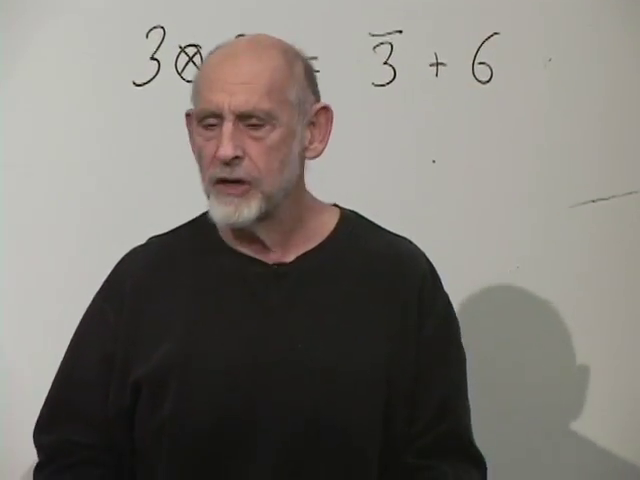
\includegraphics[width=0.68\textwidth]{lecture_04_figure_04.png}
\caption{La décomposition du produit de deux quarks en un antitriplet et un sextet.}
\lectureframe{00:39:33}
\end{figure}

On peut représenter explicitement l’antitriplet en contractant deux indices de quark avec le tenseur epsilon invariant :
\begin{equation}
(qq)^k_{\bar 3}
=\frac{1}{\sqrt2}\epsilon^{kij}q_iq_j.
\end{equation}
Cet objet a trois composantes et se transforme comme un antiquark. Les six combinaisons symétriques forment le sextet. Cela ne signifie pas que deux quarks deviennent dynamiquement un antiquark ; cela signifie qu’un secteur de leur fonction d’onde de couleur suit la même loi de transformation qu’un antiquark.

\subsection{Un quark et un antiquark : \texorpdfstring{\(\boldsymbol 3\otimes\bar{\boldsymbol 3}\)}{3 x anti-3}}

Un état de couleur quark--antiquark peut être représenté par une matrice \(3\times3\) \(M_i{}^j=q_i\bar q^j\). Toute matrice de ce type se décompose de manière unique en une partie proportionnelle à sa trace et une partie sans trace :
\begin{equation}
M=\frac{\operatorname{tr}M}{3}\boldsymbol 1
+\left(M-\frac{\operatorname{tr}M}{3}\boldsymbol 1\right).
\end{equation}
La trace est une composante invariante unique, et la partie sans trace en a huit. Par conséquent,
\begin{equation}
\boldsymbol 3\otimes\bar{\boldsymbol 3}
=\boldsymbol 1\oplus\boldsymbol 8.
\label{eq:l4-three-times-threebar}
\end{equation}
À un facteur de normalisation près, le singulet est
\begin{equation}
\ket{1}_{q\bar q}
=\frac{1}{\sqrt3}
(\ket{r\bar r}+\ket{g\bar g}+\ket{b\bar b}).
\end{equation}
Il ne peut se transformer en aucun autre état, car il est invariant. Les huit autres combinaisons linéaires se mélangent entre elles. Elles forment la représentation adjointe, celle-là même selon laquelle se transforment les huit générateurs.

\subsection{Trois quarks}

Ajoutons un troisième quark à l’équation~\eqref{eq:l4-three-times-three}. La branche antitriplet donne
\begin{equation}
\bar{\boldsymbol 3}\otimes\boldsymbol 3
=\boldsymbol 1\oplus\boldsymbol 8,
\end{equation}
Le produit de trois quarks contient donc un singulet. La décomposition complète est
\begin{equation}
\boldsymbol 3\otimes\boldsymbol 3\otimes\boldsymbol 3
=\boldsymbol 1\oplus\boldsymbol 8\oplus\boldsymbol 8
\oplus\boldsymbol{10}.
\label{eq:l4-three-quark-full}
\end{equation}
Le singulet de couleur est la combinaison entièrement antisymétrique rouge--vert--bleu,
\begin{equation}
\ket{1}_{qqq}
=\frac{1}{\sqrt6}\epsilon^{ijk}\ket{q_iq_jq_k}.
\label{eq:l4-baryon-singlet}
\end{equation}
Comme \(\epsilon^{ijk}\) s’annule dès que deux indices coïncident, chaque terme non nul contient un quark rouge, un vert et un bleu, avec des signes alternés lors des permutations.

\begin{classroomqa}
\audiencequestion{Les combinaisons non singulets sont-elles simplement peu probables, au point que l’on puisse négliger leurs probabilités ?
\lecturetimestamp{00:46:02}}
\lecturerresponse{Non. La question porte sur l’énergie, pas sur une faible probabilité. Un état non singulet isolé produirait un champ de couleur qui s’étendrait jusqu’à des distances arbitrairement grandes et, dans le régime de confinement, nécessiterait une énergie non bornée. Nous développerons plus loin la dynamique qui sous-tend cette affirmation.}
\end{classroomqa}

\subsection{L’octet de gluons}

Le champ de gluons se transforme comme l’octet de l’équation~\eqref{eq:l4-three-times-threebar}. Du point de vue de la couleur, il porte un indice de triplet et un indice d’antitriplet, dont on a retiré la trace singulet. Schématiquement,
\begin{equation}
q\sim\boldsymbol 3,
\qquad
\bar q\sim\bar{\boldsymbol 3},
\qquad
G\sim\boldsymbol 8.
\end{equation}
Ces symboles désignent des lois de transformation ; les particules ne sont pas littéralement égales aux nombres trois et huit.

La neuvième combinaison de couleur quark--antiquark, proportionnelle à l’identité, est un singulet et ne se mélange pas à l’octet. Il est donc cohérent de l’omettre mathématiquement : un champ de jauge \(SU(3)\) est sans trace et possède huit composantes, au lieu des neuf d’un champ de jauge \(U(3)\).

\begin{classroomqa}
\audiencequestion{Pourquoi la nature omet-elle le gluon singulet supplémentaire ?
\lecturetimestamp{00:49:00}}
\lecturerresponse{La réponse immédiate, du point de vue de la théorie des groupes, est que le singulet forme un secteur invariant distinct ; l’octet est donc fermé de façon cohérente sans lui. La raison plus profonde du choix de \(SU(3)\) plutôt que de \(U(3)\) n’est pas établie ici ; elle relève de la structure de jauge déduite de la phénoménologie de la QCD.}
\end{classroomqa}

\section{Les singulets de couleur comme hadrons}

Les particules libres de masse finie de l’interaction forte sont des singulets de couleur. Cela ne rend pas les quarks ou les gluons irréels ; cela signifie qu’ils n’existent pas comme particules asymptotiques isolées. Les configurations élémentaires qui forment des singulets sont
\begin{equation}
qqq,
\qquad
q\bar q,
\qquad
GG\ \text{and higher gluonic products}.
\end{equation}
Elles conduisent respectivement aux baryons, aux mésons et aux boules de glu. Des produits de plusieurs objets déjà neutres en couleur le sont bien sûr aussi ; on peut donc construire des états multihadrons plus complexes à partir de ces constituants.

\begin{classroomqa}
\audiencequestion{Comment appelle-t-on les singulets de trois quarks et de quark--antiquark, et les gluons peuvent-ils aussi former des singulets ?
\lecturetimestamp{00:51:38}}
\lecturerresponse{Un singulet de trois quarks est un baryon ; un singulet quark--antiquark est un méson. Les gluons peuvent eux aussi se combiner en singulets de couleur. Ces états de l’interaction forte, les plus simples de ce type, sont appelés boules de glu ; ils peuvent faire intervenir plus de deux gluons.}
\end{classroomqa}

Trois quarks de spin un demi se combinent toujours en un spin total demi-entier, même si le moment cinétique orbital peut modifier le demi-entier obtenu. Les mésons quark--antiquark ont un spin entier. Les boules de glu purement gluoniques ont elles aussi un spin entier.

Pour deux gluons, la première affirmation au tableau ne donne qu’un décompte :
\begin{equation}
8\times8=1+63.
\end{equation}
Il y a en tout soixante-quatre états de couleur ; une combinaison est un singulet et les soixante-trois autres appartiennent à des secteurs non singulets.

\begin{figure}[htbp]
\centering
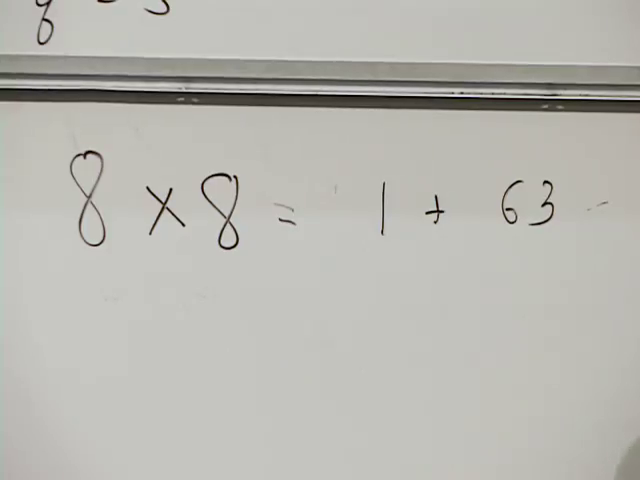
\includegraphics[width=0.68\textwidth]{lecture_04_figure_05.png}
\caption{Décompte au tableau des états à deux gluons : un singulet parmi soixante-quatre états.}
\lectureframe{00:53:44}
\end{figure}

La décomposition complète en représentations irréductibles est
\begin{equation}
\boldsymbol 8\otimes\boldsymbol 8
=\boldsymbol 1\oplus\boldsymbol 8_S\oplus\boldsymbol 8_A
\oplus\boldsymbol{10}\oplus\overline{\boldsymbol{10}}
\oplus\boldsymbol{27}.
\label{eq:l4-eight-times-eight}
\end{equation}
Les dimensions s’additionnent correctement :
\begin{equation}
1+8+8+10+10+27=64.
\end{equation}
Les deux octets sont des sous-espaces invariants distincts, l’un symétrique et l’autre antisymétrique sous l’échange des deux facteurs adjoints. Le singulet est le canal de couleur à deux gluons à partir duquel peut se former un état de boule de glu.
\editorialnote{Le tableau indique d’abord seulement \(8\times8=1+63\). L’échange ultérieur en classe donne les dimensions irréductibles énumérées ; les barres et les indices de symétrie, dans la notation usuelle de \(SU(3)\), sont rétablis ici.}

\subsection{Pourquoi les charges électriques observables sont entières}

Les charges des quarks sont de deux types :
\begin{equation}
Q_{\mathrm{up\text{-}like}}=+\frac23,
\qquad
Q_{\mathrm{down\text{-}like}}=-\frac13.
\end{equation}
La charge totale de trois quarks est donc entière : \(-1,0,+1,\text{ or }+2\), selon le nombre de quarks de type haut. De même, la charge d’un quark et d’un antiquark vaut \(0\) ou \(\pm1\). Les gluons ne portent pas de charge électrique. Ainsi, les singulets de couleur élémentaires construits à partir des représentations de quarks observées ont une charge électrique entière, même si leurs constituants portent des charges fractionnaires.

\begin{classroomqa}
\audiencequestion{Quelle est la charge électrique du quark étrange ?
\lecturetimestamp{00:56:08}}
\lecturerresponse{Il est de type bas, donc sa charge est \(-1/3\). Les trois familles reproduisent le même schéma de charges : \((u,d)\), \((c,s)\) et \((t,b)\), avec des charges \(+2/3\) et \(-1/3\) dans chaque paire.}
\end{classroomqa}

Pour ce contenu en particules, le caractère singulet de couleur et l’intégralité de la charge électrique sont étroitement liés, mais ne sont pas des énoncés mathématiques identiques. L’intégralité repose également sur les attributions de charge électrique particulières du modèle standard qui viennent d’être données.

\begin{classroomqa}
\audiencequestion{Un état singulet de couleur est-il un état intriqué, et cela a-t-il la même portée qu’une paire intriquée dans une expérience de Bell ?
\lecturetimestamp{00:56:58}}
\lecturerresponse{La fonction d’onde de couleur du singulet est bien intriquée : c’est une superposition cohérente, et non un produit d’états de couleur individuellement définis. En principe, ses constituants peuvent être séparés, mais le confinement rend cette séparation de plus en plus coûteuse et finit par produire de nouveaux hadrons. Ce n’est donc pas un système commode pour une manipulation de type Bell, même si l’état est intriqué.}
\end{classroomqa}

\section{Sens des équations de produit tensoriel}

Il convient maintenant d’expliquer plus concrètement les tables de multiplication. Soient \(\psi_i\) et \(\phi_j\) des opérateurs qui créent deux objets de spin un demi ; ils peuvent décrire deux espèces, comme un électron et un proton, ou deux exemplaires d’une même espèce, avec prise en compte des statistiques appropriées. Chaque indice prend deux valeurs. Les quatre produits
\begin{equation}
\psi_\uparrow\phi_\uparrow,
\quad
\psi_\uparrow\phi_\downarrow,
\quad
\psi_\downarrow\phi_\uparrow,
\quad
\psi_\downarrow\phi_\downarrow
\end{equation}
engendrent l’espace produit tensoriel.

Si un élément du groupe agit comme \(U\) sur chaque facteur, il agit comme \(U\otimes U\) sur leur produit. En composantes,
\begin{equation}
\psi_i\phi_j
\longmapsto
U_i{}^kU_j{}^\ell\psi_k\phi_\ell.
\label{eq:l4-product-action}
\end{equation}
Il s’agit d’une représentation de dimension quatre, mais elle est réductible. La combinaison antisymétrique
\begin{equation}
\frac{1}{\sqrt2}
(\psi_\uparrow\phi_\downarrow
-\psi_\downarrow\phi_\uparrow)
\end{equation}
se transforme en elle-même, tandis que les trois combinaisons symétriques se transforment entre elles. Dans la base adaptée à ces combinaisons, chaque matrice de la représentation produit prend une forme diagonale par blocs :
\begin{equation}
D_{2\otimes2}(g)
\sim
\begin{pmatrix}
1&0\\
0&D_3(g)
\end{pmatrix}.
\label{eq:l4-spin-block-diagonal}
\end{equation}

\begin{classroomqa}
\audiencequestion{Quelle opération représente une équation telle que \(\boldsymbol 3\otimes\boldsymbol 3=\bar{\boldsymbol 3}\oplus\boldsymbol 6\) ?
\lecturetimestamp{00:57:51}}
\lecturerresponse{Le membre de gauche construit l’espace d’états composé. Le groupe agit sur les deux facteurs et mélange donc les états de la base produit. Le membre de droite indique qu’un changement de base sépare ces états en ensembles invariants : trois combinaisons antisymétriques qui se transforment comme un antitriplet et six combinaisons symétriques qui se transforment comme un sextet. Le signe plus désigne une somme directe de secteurs, et non une addition numérique ordinaire.}
\end{classroomqa}

\begin{classroomqa}
\audiencequestion{Comment sait-on que les neuf états se décomposent en \(3+6\) ou en \(1+8\), plutôt que, par exemple, en \(2+7\) ?
\lecturetimestamp{01:04:39}}
\lecturerresponse{Le seul décompte des dimensions ne permet pas de déterminer la décomposition. Il faut connaître les représentations irréductibles de \(SU(3)\) et construire des sous-espaces invariants, par exemple en symétrisant ou en antisymétrisant les indices, ou en séparant les parties avec et sans trace. Une classification complète exige davantage de théorie des groupes ; ici, nous n’utilisons que les représentations nécessaires pour les quarks et les gluons.}
\end{classroomqa}

Le tenseur epsilon invariant rend transparente la construction du singulet. Pour \(SU(2)\),
\begin{equation}
\epsilon_{ij}U^i{}_kU^j{}_\ell
=(\det U)\epsilon_{k\ell}
=\epsilon_{k\ell}.
\end{equation}
Par conséquent, \(\epsilon_{ij}\psi^i\phi^j\) est invariant. Pour \(SU(3)\), la version à trois indices donne
\begin{equation}
\epsilon_{ijk}U^i{}_aU^j{}_bU^k{}_c
=(\det U)\epsilon_{abc}
=\epsilon_{abc},
\end{equation}
ce qui établit l’invariance de l’état à trois quarks de l’équation~\eqref{eq:l4-baryon-singlet}.

\begin{classroomqa}
\audiencequestion{Peut-on montrer explicitement pourquoi le singulet ne se transforme pas ?
\lecturetimestamp{01:07:18}}
\lecturerresponse{Oui. Contractez tous les indices fondamentaux avec le tenseur epsilon complètement antisymétrique. Sous la transformation, le produit des matrices multiplie epsilon par \(\det U\). Pour une matrice spéciale unitaire, ce déterminant vaut un ; l’état contracté reste donc inchangé. Dans \(SU(2)\), cela démontre l’invariance du singulet de deux spins ; dans \(SU(3)\), celle du singulet rouge--vert--bleu à trois quarks.}
\end{classroomqa}

\begin{classroomqa}
\audiencequestion{Quelle est la décomposition complète de deux octets de gluons ?
\lecturetimestamp{01:09:24}}
\lecturerresponse{C’est la décomposition de l’équation~\eqref{eq:l4-eight-times-eight} : un singulet, deux octets, un décuplet, un antidécuplet et une représentation de dimension vingt-sept. Il existe exactement une combinaison singulet de couleur des deux indices d’octet.}
\end{classroomqa}

\begin{classroomqa}
\audiencequestion{Quelle est la décomposition complète correspondante pour trois quarks ?
\lecturetimestamp{01:11:51}}
\lecturerresponse{Le résultat essentiel du point de vue physique est qu’elle contient un singulet. Le décompte complet donne l’équation~\eqref{eq:l4-three-quark-full} : un singulet, deux octets et un décuplet, soit en tout \(1+8+8+10=27\) états.\editorialnote{Le conférencier ne se rappelle pas la décomposition complète de \(3\otimes3\otimes3\) pendant l’échange. La complétion usuelle est fournie explicitement et signalée comme telle, sans être attribuée à la réponse orale.}}
\end{classroomqa}

La même idée s’étend à l’espace de deux gluons. Dans la base produit naïve,
\(SU(3)\) agit au moyen de matrices \(64\times64\). Dans une base adaptée aux composantes irréductibles, ces matrices sont diagonales par blocs,
\begin{equation}
\begin{aligned}
D_{8\otimes8}(g)
&\sim
\operatorname{diag}\bigl(
1,D_{8_S}(g),D_{8_A}(g),
\\
&\hspace{4.8em}
D_{10}(g),D_{\overline{10}}(g),D_{27}(g)
\bigr).
\end{aligned}
\end{equation}
Aucun bloc ne se mélange à un autre, bien que les états se mélangent entre eux au sein de chaque bloc.

\begin{classroomqa}
\audiencequestion{La décomposition en produit tensoriel consiste-t-elle simplement à changer de base pour rendre diagonale par blocs la grande matrice de représentation ?
\lecturetimestamp{01:12:02}}
\lecturerresponse{Exactement. Pour deux spins, la matrice de dimension quatre devient un bloc singulet de dimension un et un bloc triplet de dimension trois. Pour deux gluons, la matrice de dimension soixante-quatre devient des blocs de dimensions \(1,8,8,10,10,\text{ and }27\). Chaque bloc est stable sous toute transformation du groupe.}
\end{classroomqa}

\begin{classroomqa}
\audiencequestion{Y a-t-il un nom pour l’une de ces parties stables à l’intérieur de l’espace produit tensoriel complet ?
\lecturetimestamp{01:14:55}}
\lecturerresponse{C’est un sous-espace invariant qui porte une sous-représentation. Lorsqu’il ne peut pas être décomposé davantage, il porte une représentation irréductible, ou irréductible. Le produit tensoriel complet est la somme directe de ces composantes irréductibles.\editorialnote{Le terme demandé reste sans réponse dans la salle. La réponse fournit la terminologie usuelle de la théorie des représentations.}}
\end{classroomqa}

\begin{classroomqa}
\audiencequestion{Lorsque les représentations de dimension dix non singulets et d’autres représentations sont dites inexistantes, cela signifie-t-il qu’il faut les ignorer complètement ?
\lecturetimestamp{01:15:36}}
\lecturerresponse{Ce sont des secteurs de couleur légitimes, qui interviennent dans les calculs intermédiaires, mais ils n’apparaissent pas comme des particules isolées d’énergie finie en laboratoire. C’est le confinement, et non une défaillance de la théorie des représentations, qui les empêche de devenir des états asymptotiques libres.}
\end{classroomqa}

\section{De l’idée de couleur de Nambu au confinement}

L’idée de couleur précède la formulation définitive de la QCD. Dès les années 1960, Yoichiro Nambu avait compris qu’un nombre quantique caché à trois valeurs pouvait résoudre un problème frappant : les quarks portent une charge électrique fractionnaire, et pourtant aucune particule libre de charge fractionnaire n’est observée. Si les états physiques sont contraints d’être des singulets de couleur, les quarks apparaissent dans les combinaisons de charge entière décrites plus haut. Reste une question dynamique : quelles forces contraignent tous les états libres d’énergie finie à être des singulets ?

Commençons par l’analogie électromagnétique. Une charge et une charge opposée s’attirent. Les rapprocher abaisse l’énergie ; rapprocher des charges de même signe nécessite un travail. Le champ lui-même stocke une énergie positive,
\begin{equation}
E_{\mathrm{field}}
=\frac12\int d^3x\,\boldsymbol E^2
\end{equation}
dans les unités électrostatiques usuelles. Une charge nette produit un champ qui s’étend loin au-delà du système, tandis qu’une paire neutre fortement liée ne produit qu’un champ dipolaire de courte portée. La neutralisation élimine donc l’énergie du champ à l’extérieur.

Imaginons que l’on augmente énormément le couplage électromagnétique. Le coût énergétique du champ associé à une charge nette deviendrait si élevé que les objets de basse énergie seraient presque toujours neutres, et que l’extraction d’un constituant chargé pourrait devenir prohibitive. Nambu a transposé cette intuition à la couleur : les huit charges de couleur sont les sources de huit champs de gluons ; une grande énergie du champ de couleur pourrait donc interdire les états non singulets isolés.

Cette intuition est essentiellement juste, mais la QCD comporte une caractéristique nouvelle décisive. Le photon ne porte pas de charge électrique, tandis que le gluon porte une charge de couleur. Le photon n’est pas une source du champ électromagnétique classique, et les équations de Maxwell sont linéaires : deux ondes électromagnétiques se superposent et se traversent. Un gluon se transforme selon l’octet de couleur ; les gluons sont donc des sources les uns pour les autres et interagissent entre eux. Même différentes parties d’un même champ de gluons interagissent. Le champ de jauge non abélien est donc non linéaire.

\subsection{Tubes de flux et potentiel linéaire}

À longue distance, l’auto-interaction des gluons empêche le flux de couleur de s’étaler comme un champ dipolaire électrique ordinaire. Le flux est comprimé dans un tube qui relie un quark à un antiquark. L’intensité du champ et la section transversale d’un long tube sont approximativement constantes ; le tube stocke donc une énergie approximativement constante par unité de longueur. Si \(\sigma\) désigne cette tension de corde, alors
\begin{equation}
V(R)\simeq\sigma R+\text{constant}
\qquad (R\ \text{large}).
\label{eq:l4-linear-potential}
\end{equation}

\begin{figure}[htbp]
\centering
\includegraphics[width=0.78\textwidth]{lecture_04_figure_06.png}
\caption{Flux de couleur regroupé dans un long tube entre un quark et un antiquark.}
\lectureframe{01:31:35}
\end{figure}

C’est plus fort que le potentiel de Coulomb, dont la valeur absolue décroît comme \(1/R\). Éloigner davantage les sources de couleur n’affaiblit pas indéfiniment la force ; cela allonge le tube et ajoute continuellement de l’énergie. Une charge de couleur isolée dans un volume infini nécessiterait un tube sans fin et donc une énergie non bornée. Voilà ce que signifie concrètement l’affirmation selon laquelle seuls les singulets de couleur sont des états asymptotiques d’énergie finie.
\editorialnote{La notation de la tension de corde et l’expression explicite du potentiel à longue distance quantifient l’affirmation de la source selon laquelle un tube de flux uniforme porte une énergie uniforme par unité de longueur.}

\subsection{Rupture de corde et jets}

Supposons qu’une collision à haute énergie frappe un quark à l’intérieur d’un méson. Le quark commence à s’éloigner, mais le tube de flux s’étire derrière lui. Il peut perdre son énergie cinétique et être ramené vers l’arrière. Le plus souvent, dès que l’énergie stockée dans le champ devient suffisante, le vide produit une nouvelle paire quark--antiquark. Le nouvel antiquark met fin au flux attaché au quark qui s’échappe, tandis que le nouveau quark met fin au flux attaché à l’antiquark initial. Un singulet étiré devient deux singulets plus courts,
\begin{equation}
(q\bar q)_{\mathrm{stretched}}
\longrightarrow
(q\bar q)+(q\bar q).
\label{eq:l4-string-breaking}
\end{equation}

\begin{figure}[htbp]
\centering
\includegraphics[width=0.78\textwidth]{lecture_04_figure_07.png}
\caption{La création d’une paire rompt un tube de flux étiré en deux tubes singulets de couleur.}
\lectureframe{01:34:52}
\end{figure}

\begin{classroomqa}
\audiencequestion{Si un quark frappé possède assez d’énergie pour continuer à étirer le tube, que peut-il se passer d’autre que son retour vers l’arrière ?
\lecturetimestamp{01:33:50}}
\lecturerresponse{Le tube peut se rompre par création d’une paire quark--antiquark. Son énergie devient la masse et l’énergie cinétique de la nouvelle paire. Les extrémités se reconnectent en deux singulets ; le processus crée donc des mésons supplémentaires plutôt qu’un quark isolé.}
\end{classroomqa}

Si l’un de ces partons porte encore une grande quantité de mouvement, le processus se répète. Il en résulte une cascade de hadrons singulets de couleur, collimatés autour de la direction du parton initial : un jet. Cette conversion de quarks et de gluons énergétiques en hadrons s’appelle l’hadronisation. On déduit l’existence de l’objet coloré initial à partir du jet ; on ne l’observe jamais isolément.

\begin{classroomqa}
\audiencequestion{La rupture de corde ne produit-elle que des mésons, ou d’autres hadrons peuvent-ils apparaître dans le jet ?
\lecturetimestamp{01:35:20}}
\lecturerresponse{D’autres hadrons peuvent tout à fait apparaître. La seule exigence de couleur est que les objets observables finaux soient des singulets. Les mésons constituent le modèle le plus simple pour une rupture, mais des baryons, des antibaryons et des combinaisons singulets plus complexes peuvent également être produits.}
\end{classroomqa}

Trois quarks peuvent terminer leurs flux dans une jonction singulet de couleur. La configuration à trois branches est le pendant dynamique du tenseur epsilon antisymétrique dans l’équation~\eqref{eq:l4-baryon-singlet} : aucun flux net de couleur ne s’échappe du baryon dans son ensemble.

\begin{figure}[htbp]
\centering
\includegraphics[width=0.72\textwidth]{lecture_04_figure_08.png}
\caption{Jonction de flux de couleur à trois branches pour un baryon, sous le schéma de rupture de corde d’un méson.}
\lectureframe{01:36:12}
\end{figure}

\section{Champs de jauge, charges conservées et modèle standard}

À ce stade, on peut reconnaître une théorie de jauge au fait qu’une charge conservée est la source d’un champ de type photon. La charge électrique est la source du champ électromagnétique ; les huit charges de couleur sont les sources des huit champs de gluons. Dans la formulation plus profonde, la symétrie devient locale et l’on introduit une connexion qui compare les états internes en des points voisins de l’espace-temps, mais cette construction n’est pas nécessaire pour comprendre le tableau du confinement présenté ici.
\editorialnote{La formulation en termes de symétrie locale est le sens plus profond usuel de la théorie de jauge, évoqué dans la source mais délibérément reporté.}

La symétrie, la charge conservée et le flux sont étroitement liés. Si les lignes de champ ne peuvent se terminer que sur des charges, une source ne peut pas simplement disparaître alors que son flux reste attaché à rien. Son champ lointain ne peut pas non plus disparaître instantanément en totalité, car les variations du champ se propagent de manière causale. Sous forme locale, la même physique s’exprime par une équation de continuité,
\begin{equation}
\frac{\partial\rho}{\partial t}
+\boldsymbol\nabla\cdot\boldsymbol j=0,
\end{equation}
qui indique qu’une charge ne peut quitter une région qu’en traversant sa frontière. L’argument des lignes de champ est la représentation géométrique de cette loi locale de conservation.

Nous pouvons maintenant situer ce résultat dans le modèle standard. La couleur apporte les huit générateurs de \(SU(3)\) et leurs huit champs de gluons. Le secteur abélien fournit un générateur et un champ de jauge. Trois autres générateurs appartiennent à un groupe \(SU(2)\) supplémentaire, et non au moment cinétique orbital ordinaire. Avant la brisure de symétrie, la structure de jauge est
\begin{equation}
SU(3)_c\times SU(2)_L\times U(1)_Y,
\end{equation}
avec \(8+3+1=12\) générateurs. Il faut ensuite comprendre le secteur électrofaible \(SU(2)\), puis le champ de Higgs et la manière dont émergent le photon observé, \(W^\pm\) et \(Z\).
\editorialnote{La source compte le photon avec les huit gluons et décrit le facteur restant comme \(SU(2)\times U(1)\). Dans le modèle standard non brisé, le facteur abélien est l’hypercharge \(U(1)_Y\) ; le photon n’apparaît qu’après le mélange électrofaible.}

La chaîne centrale est maintenant complète. Les groupes abstraits agissent par l’intermédiaire de représentations ; les générateurs infinitésimaux sont les charges conservées ; les quarks, les antiquarks et les gluons occupent les représentations \(\boldsymbol 3\),
\(\bar{\boldsymbol 3}\) et \(\boldsymbol 8\) ; les produits tensoriels identifient les hadrons singulets ; et le champ non linéaire des gluons fait de la sélection des singulets le phénomène physique du confinement.
